\documentclass{standalone}
\usepackage{tikz}
\usetikzlibrary{patterns}
\usetikzlibrary{positioning}
\usetikzlibrary{patterns, positioning}
\usetikzlibrary{shapes.misc}
\usepackage[outline]{contour}
\contourlength{1.5pt} 


\begin{document}
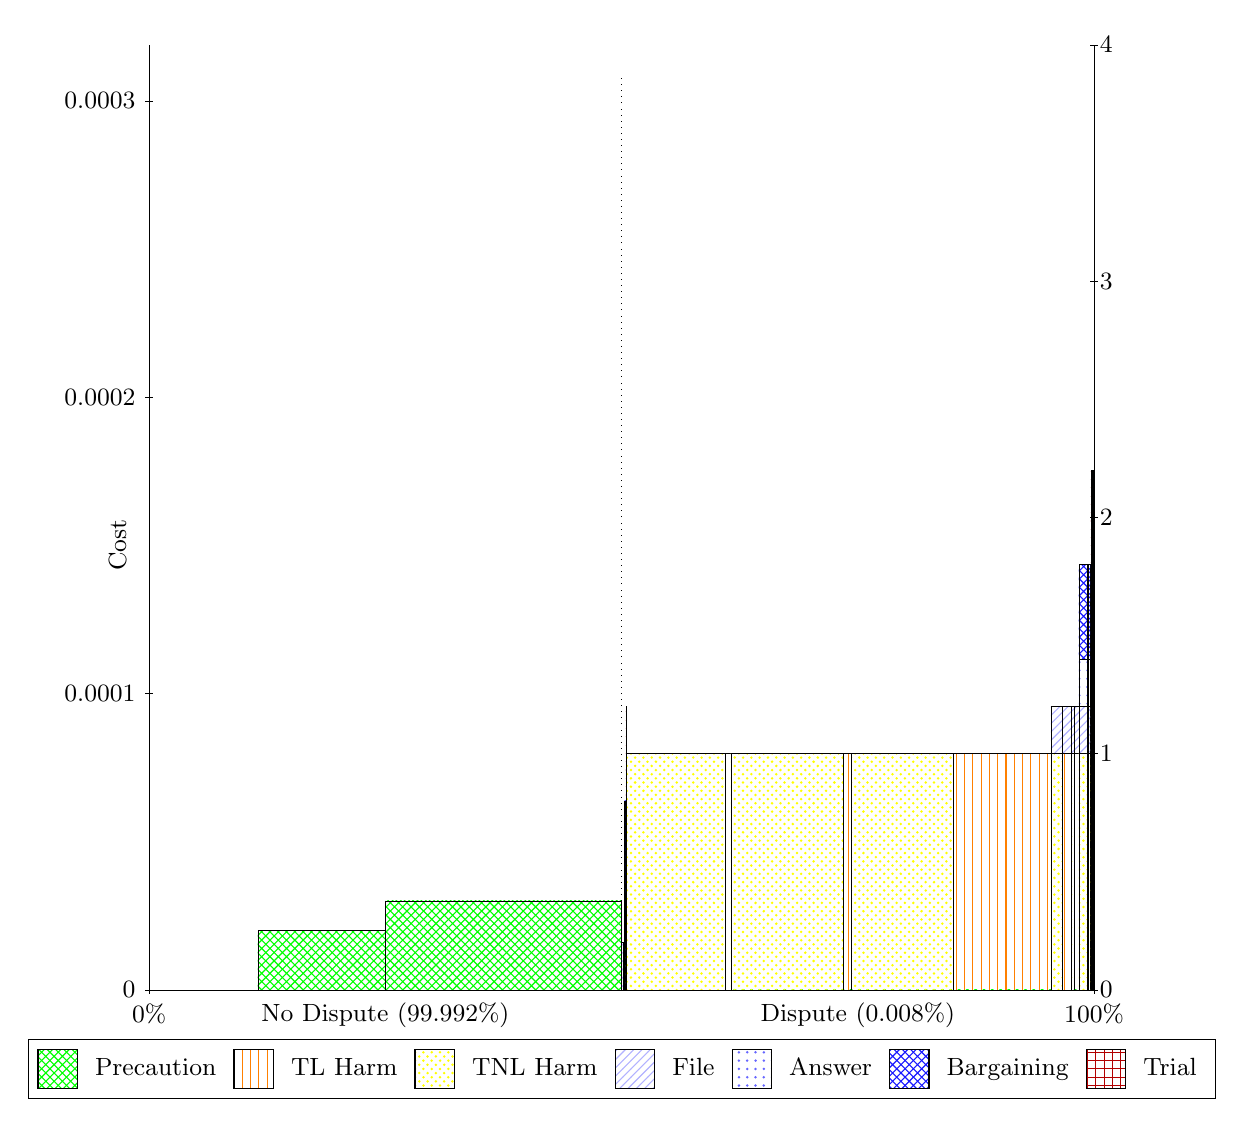
\begin{tikzpicture}
\draw[pattern=crosshatch, pattern color=green,draw=black,very thin] (2.8801,2.5) rectangle (4.5,3.2527);
\draw[pattern=crosshatch, pattern color=green,draw=black,very thin] (4.5,2.5) rectangle (7.5,3.629);
\draw[pattern=north east lines, pattern color=blue!30,draw=black,very thin] (7.5,2.5) rectangle (7.5257,3.1);
\draw[pattern=crosshatch, pattern color=green,draw=black,very thin] (7.5257,2.5) rectangle (7.5385,2.5001);
\draw[pattern=north east lines, pattern color=blue!30,draw=black,very thin] (7.5257,2.5001) rectangle (7.5385,3.1001);
\draw[pattern=north east lines, pattern color=blue!30,draw=black,very thin] (7.5385,2.5) rectangle (7.5506,3.1);
\draw[pattern=dots,  pattern color=blue!60,draw=black,very thin] (7.5385,3.1) rectangle (7.5506,3.7);
\draw[pattern=crosshatch,      pattern color=blue!90,draw=black,very thin] (7.5385,3.7) rectangle (7.5506,4.9);
\draw[pattern=crosshatch, pattern color=green,draw=black,very thin] (7.5506,2.5) rectangle (7.5547,2.5001);
\draw[pattern=north east lines, pattern color=blue!30,draw=black,very thin] (7.5506,2.5001) rectangle (7.5547,3.1001);
\draw[pattern=dots,  pattern color=blue!60,draw=black,very thin] (7.5506,3.1001) rectangle (7.5547,3.7001);
\draw[pattern=crosshatch,      pattern color=blue!90,draw=black,very thin] (7.5506,3.7001) rectangle (7.5547,4.9001);
\draw[pattern=north east lines, pattern color=blue!30,draw=black,very thin] (7.5547,2.5) rectangle (7.5573,3.1);
\draw[pattern=dots,  pattern color=blue!60,draw=black,very thin] (7.5547,3.1) rectangle (7.5573,3.7);
\draw[pattern=crosshatch,      pattern color=blue!90,draw=black,very thin] (7.5547,3.7) rectangle (7.5573,4.9);
\draw[pattern=grid,            pattern color=red!70!black,draw=black,very thin] (7.5547,4.9) rectangle (7.5573,6.1);
\draw[pattern=crosshatch, pattern color=green,draw=black,very thin] (7.5573,2.5) rectangle (7.5591,2.5001);
\draw[pattern=north east lines, pattern color=blue!30,draw=black,very thin] (7.5573,2.5001) rectangle (7.5591,3.1001);
\draw[pattern=dots,  pattern color=blue!60,draw=black,very thin] (7.5573,3.1001) rectangle (7.5591,3.7001);
\draw[pattern=crosshatch,      pattern color=blue!90,draw=black,very thin] (7.5573,3.7001) rectangle (7.5591,4.9001);
\draw[pattern=grid,            pattern color=red!70!black,draw=black,very thin] (7.5573,4.9001) rectangle (7.5591,6.1001);
\draw[pattern=crosshatch dots, pattern color=yellow,draw=black,very thin] (7.5591,2.5) rectangle (8.8203,5.5);
\draw[pattern=vertical lines, pattern color=orange,draw=black,very thin] (8.8203,2.5) rectangle (8.8862,5.5);
\draw[pattern=crosshatch, pattern color=green,draw=black,very thin] (8.8862,2.5) rectangle (10.31,2.5001);
\draw[pattern=crosshatch dots, pattern color=yellow,draw=black,very thin] (8.8862,2.5001) rectangle (10.31,5.5001);
\draw[pattern=crosshatch, pattern color=green,draw=black,very thin] (10.31,2.5) rectangle (10.42,2.5001);
\draw[pattern=vertical lines, pattern color=orange,draw=black,very thin] (10.31,2.5001) rectangle (10.42,5.5001);
\draw[pattern=crosshatch, pattern color=green,draw=black,very thin] (10.42,2.5) rectangle (11.714,2.5001);
\draw[pattern=crosshatch dots, pattern color=yellow,draw=black,very thin] (10.42,2.5001) rectangle (11.714,5.5001);
\draw[pattern=crosshatch, pattern color=green,draw=black,very thin] (11.714,2.5) rectangle (12.95,2.5001);
\draw[pattern=vertical lines, pattern color=orange,draw=black,very thin] (11.714,2.5001) rectangle (12.95,5.5001);
\draw[pattern=crosshatch dots, pattern color=yellow,draw=black,very thin] (12.95,2.5) rectangle (13.1,5.5);
\draw[pattern=north east lines, pattern color=blue!30,draw=black,very thin] (12.95,5.5) rectangle (13.1,6.1);
\draw[pattern=vertical lines, pattern color=orange,draw=black,very thin] (13.1,2.5) rectangle (13.207,5.5);
\draw[pattern=north east lines, pattern color=blue!30,draw=black,very thin] (13.1,5.5) rectangle (13.207,6.1);
\draw[pattern=crosshatch, pattern color=green,draw=black,very thin] (13.207,2.5) rectangle (13.243,2.5001);
\draw[pattern=crosshatch dots, pattern color=yellow,draw=black,very thin] (13.207,2.5001) rectangle (13.243,5.5001);
\draw[pattern=north east lines, pattern color=blue!30,draw=black,very thin] (13.207,5.5001) rectangle (13.243,6.1001);
\draw[pattern=crosshatch, pattern color=green,draw=black,very thin] (13.243,2.5) rectangle (13.307,2.5001);
\draw[pattern=vertical lines, pattern color=orange,draw=black,very thin] (13.243,2.5001) rectangle (13.307,5.5001);
\draw[pattern=north east lines, pattern color=blue!30,draw=black,very thin] (13.243,5.5001) rectangle (13.307,6.1001);
\draw[pattern=crosshatch dots, pattern color=yellow,draw=black,very thin] (13.307,2.5) rectangle (13.408,5.5);
\draw[pattern=north east lines, pattern color=blue!30,draw=black,very thin] (13.307,5.5) rectangle (13.408,6.1);
\draw[pattern=dots,  pattern color=blue!60,draw=black,very thin] (13.307,6.1) rectangle (13.408,6.7);
\draw[pattern=crosshatch,      pattern color=blue!90,draw=black,very thin] (13.307,6.7) rectangle (13.408,7.9);
\draw[pattern=vertical lines, pattern color=orange,draw=black,very thin] (13.408,2.5) rectangle (13.428,5.5);
\draw[pattern=north east lines, pattern color=blue!30,draw=black,very thin] (13.408,5.5) rectangle (13.428,6.1);
\draw[pattern=dots,  pattern color=blue!60,draw=black,very thin] (13.408,6.1) rectangle (13.428,6.7);
\draw[pattern=crosshatch,      pattern color=blue!90,draw=black,very thin] (13.408,6.7) rectangle (13.428,7.9);
\draw[pattern=crosshatch, pattern color=green,draw=black,very thin] (13.428,2.5) rectangle (13.448,2.5001);
\draw[pattern=crosshatch dots, pattern color=yellow,draw=black,very thin] (13.428,2.5001) rectangle (13.448,5.5001);
\draw[pattern=north east lines, pattern color=blue!30,draw=black,very thin] (13.428,5.5001) rectangle (13.448,6.1001);
\draw[pattern=dots,  pattern color=blue!60,draw=black,very thin] (13.428,6.1001) rectangle (13.448,6.7001);
\draw[pattern=crosshatch,      pattern color=blue!90,draw=black,very thin] (13.428,6.7001) rectangle (13.448,7.9001);
\draw[pattern=crosshatch, pattern color=green,draw=black,very thin] (13.448,2.5) rectangle (13.46,2.5001);
\draw[pattern=vertical lines, pattern color=orange,draw=black,very thin] (13.448,2.5001) rectangle (13.46,5.5001);
\draw[pattern=north east lines, pattern color=blue!30,draw=black,very thin] (13.448,5.5001) rectangle (13.46,6.1001);
\draw[pattern=dots,  pattern color=blue!60,draw=black,very thin] (13.448,6.1001) rectangle (13.46,6.7001);
\draw[pattern=crosshatch,      pattern color=blue!90,draw=black,very thin] (13.448,6.7001) rectangle (13.46,7.9001);
\draw[pattern=crosshatch dots, pattern color=yellow,draw=black,very thin] (13.46,2.5) rectangle (13.473,5.5);
\draw[pattern=north east lines, pattern color=blue!30,draw=black,very thin] (13.46,5.5) rectangle (13.473,6.1);
\draw[pattern=dots,  pattern color=blue!60,draw=black,very thin] (13.46,6.1) rectangle (13.473,6.7);
\draw[pattern=crosshatch,      pattern color=blue!90,draw=black,very thin] (13.46,6.7) rectangle (13.473,7.9);
\draw[pattern=grid,            pattern color=red!70!black,draw=black,very thin] (13.46,7.9) rectangle (13.473,9.1);
\draw[pattern=vertical lines, pattern color=orange,draw=black,very thin] (13.473,2.5) rectangle (13.486,5.5);
\draw[pattern=north east lines, pattern color=blue!30,draw=black,very thin] (13.473,5.5) rectangle (13.486,6.1);
\draw[pattern=dots,  pattern color=blue!60,draw=black,very thin] (13.473,6.1) rectangle (13.486,6.7);
\draw[pattern=crosshatch,      pattern color=blue!90,draw=black,very thin] (13.473,6.7) rectangle (13.486,7.9);
\draw[pattern=grid,            pattern color=red!70!black,draw=black,very thin] (13.473,7.9) rectangle (13.486,9.1);
\draw[pattern=crosshatch, pattern color=green,draw=black,very thin] (13.486,2.5) rectangle (13.492,2.5001);
\draw[pattern=crosshatch dots, pattern color=yellow,draw=black,very thin] (13.486,2.5001) rectangle (13.492,5.5001);
\draw[pattern=north east lines, pattern color=blue!30,draw=black,very thin] (13.486,5.5001) rectangle (13.492,6.1001);
\draw[pattern=dots,  pattern color=blue!60,draw=black,very thin] (13.486,6.1001) rectangle (13.492,6.7001);
\draw[pattern=crosshatch,      pattern color=blue!90,draw=black,very thin] (13.486,6.7001) rectangle (13.492,7.9001);
\draw[pattern=grid,            pattern color=red!70!black,draw=black,very thin] (13.486,7.9001) rectangle (13.492,9.1001);
\draw[pattern=crosshatch, pattern color=green,draw=black,very thin] (13.492,2.5) rectangle (13.5,2.5001);
\draw[pattern=vertical lines, pattern color=orange,draw=black,very thin] (13.492,2.5001) rectangle (13.5,5.5001);
\draw[pattern=north east lines, pattern color=blue!30,draw=black,very thin] (13.492,5.5001) rectangle (13.5,6.1001);
\draw[pattern=dots,  pattern color=blue!60,draw=black,very thin] (13.492,6.1001) rectangle (13.5,6.7001);
\draw[pattern=crosshatch,      pattern color=blue!90,draw=black,very thin] (13.492,6.7001) rectangle (13.5,7.9001);
\draw[pattern=grid,            pattern color=red!70!black,draw=black,very thin] (13.492,7.9001) rectangle (13.5,9.1001);
\draw[black,very thin] (1.5,2.5) -- (1.5,14.5);
\node[font=\small,rotate=90,text=black, anchor=center] at (1.1, 8.145) {Cost};
\draw[black,very thin] (1.45,2.5) -- (1.55,2.5);
\node[font=\small,text=black, anchor=east] at (1.45, 2.5) {0};
\draw[black,very thin] (1.45,6.2633) -- (1.55,6.2633);
\node[font=\small,text=black, anchor=east] at (1.45, 6.2633) {0.0001};
\draw[black,very thin] (1.45,10.027) -- (1.55,10.027);
\node[font=\small,text=black, anchor=east] at (1.45, 10.027) {0.0002};
\draw[black,very thin] (1.45,13.79) -- (1.55,13.79);
\node[font=\small,text=black, anchor=east] at (1.45, 13.79) {0.0003};

\draw[black,dotted,very thin] (7.5,2.86) -- (7.5,14.14);
\draw[black,very thin] (13.5,2.5) -- (13.5,14.5);
\draw[black,very thin] (13.45,2.5) -- (13.55,2.5);
\node[font=\small,text=black, anchor=west] at (13.45, 2.5) {0};
\draw[black,very thin] (13.45,5.5) -- (13.55,5.5);
\node[font=\small,text=black, anchor=west] at (13.45, 5.5) {1};
\draw[black,very thin] (13.45,8.5) -- (13.55,8.5);
\node[font=\small,text=black, anchor=west] at (13.45, 8.5) {2};
\draw[black,very thin] (13.45,11.5) -- (13.55,11.5);
\node[font=\small,text=black, anchor=west] at (13.45, 11.5) {3};
\draw[black,very thin] (13.45,14.5) -- (13.55,14.5);
\node[font=\small,text=black, anchor=west] at (13.45, 14.5) {4};

\draw[black,very thin] (1.5,2.5) -- (13.5,2.5);
\draw[black,very thin] (1.5,2.45) -- (1.5,2.55);
\node[font=\small,text=black, anchor=north] at (1.5, 2.45) {0\%};
\draw[black,very thin] (13.5,2.45) -- (13.5,2.55);
\node[font=\small,text=black, anchor=north] at (13.5, 2.45) {100\%};

\node[font=\small,text=black,anchor=south] at (4.5, 1.9) {No\ Dispute\ (99.992\%)};
\node[font=\small,text=black,anchor=south] at (10.5, 1.9) {Dispute\ (0.008\%)};
\draw (7.5,2.5) node (B) {};
\begin{scope}[align=center]
\matrix[scale=0.5,draw=black,below=0.5cm of B,nodes={draw},column sep=0.1cm]{
\node[rectangle,draw,minimum width=0.5cm,minimum height=0.5cm,pattern=crosshatch, pattern color=green]{}; & \node[draw=none,font=\small,text=black]{Precaution}; &
\node[rectangle,draw,minimum width=0.5cm,minimum height=0.5cm,pattern=vertical lines, pattern color=orange]{}; & \node[draw=none,font=\small,text=black]{TL Harm}; &
\node[rectangle,draw,minimum width=0.5cm,minimum height=0.5cm,pattern=crosshatch dots, pattern color=yellow]{}; & \node[draw=none,font=\small,text=black]{TNL Harm}; &
\node[rectangle,draw,minimum width=0.5cm,minimum height=0.5cm,pattern=north east lines, pattern color=blue!30]{}; & \node[draw=none,font=\small,text=black]{File}; &
\node[rectangle,draw,minimum width=0.5cm,minimum height=0.5cm,pattern=dots,  pattern color=blue!60]{}; & \node[draw=none,font=\small,text=black]{Answer}; &
\node[rectangle,draw,minimum width=0.5cm,minimum height=0.5cm,pattern=crosshatch,      pattern color=blue!90]{}; & \node[draw=none,font=\small,text=black]{Bargaining}; &
\node[rectangle,draw,minimum width=0.5cm,minimum height=0.5cm,pattern=grid,            pattern color=red!70!black]{}; & \node[draw=none,font=\small,text=black]{Trial}; \\\\
};\end{scope}

\end{tikzpicture}
\end{document}